\documentclass[12pt]{article}

\usepackage[a4paper, left=2cm, right=2cm, top=2cm]{geometry}
\usepackage{graphicx}
\usepackage{float}

\title{GDD Bevy Survivor}

\begin{document}


\maketitle
\newpage

\tableofcontents
\section{Introduction}


\newpage
\section{Enemies}
What are the key features of enemies, and how do they differ from each other?
\begin{itemize}
    \item Movement: How does the enemy type move?
    \item Damage: How does the enemy type deal damage?
    \item Health: How much health does the enemy type have?
    \item Resistance: Is the enemy type resistant to something?
\end{itemize}
Each enemy type should make the player behave differently to defeat it.For each enemy type, let's ask ourselves: 
How does the player defeat this enemy type, and how is it different from the other types?\\

\noindent
The following subsections describe the different types of enemies.

\subsection{Walker}
The Walker enemy is the typical “filler” enemy and has these features.
\begin{itemize}
    \item Movement: Walks slower than the player in their direction. 
    \item Damage: Deals damage on collision with the player. 
    \item Health: Moderate amount of health. This type should be cannon fodder. 
    \item Resistance: No specific resistances.
\end{itemize}
These enemies should make the player feel a basic level of threat and keep them moving.

\subsection{Sprinter}
The Sprinter enemy is a special type of enemy, which is not as common as the Walker type.
\begin{itemize}
    \item Movement: Keeps distance from the player and then sprints toward them. 
    \item Damage: Deals damage on collision with the player and knocks them back. 
    \item Health: Moderate amount of health.
    \item Resistance: Becomes “unstoppable” while sprinting.
\end{itemize}
The player needs to actively dodge this enemy's charge, which may interrupt their planned path and force them to take a new one.

\subsection{Jumper}
The Jumper enemy is a special type of enemy, which is not as common as the Walker type.
\begin{itemize}
    \item Movement: Keeps distance from the player and jumps toward them. 
    \item Damage: Deals damage on impact and creates a zone with a special effect\\
    (e.g., slow, poison, fire, etc.).
    \item Health: Should feel tanky.
    \item Resistance: No specific resistances.
\end{itemize}
The player needs to move out of the indicated landing area and avoid stepping into it again. This may lead to tricky situations where the player must choose between walking into the puddle or into approaching enemies.

\subsection{Shooter}
The Shooter enemy is a special type of enemy, which is not as common as the Walker type.
\begin{itemize}
    \item Movement: Keeps distance from the player.  
    \item Damage: Deals damage if its projectile hits the player. 
    \item Health: Should feel squishy.
    \item Resistance: No specific resistances.
\end{itemize}
The player needs to track the shots of these enemies, forcing them to watch the whole screen and not just the nearest enemies.

\subsection{Swarm}
The Swarm enemies are a group of smaller enemies.
\begin{itemize}
    \item Movement: Moves as a group from one side of the screen to the other. 
    \item Damage: Deals damage on collision with the player.
    \item Health: Individual swarm enemies are very squishy. 
    \item Resistance: Very easy to knock back. 
\end{itemize}
An incoming swarm of enemies flying quickly toward the player may create an “oh no” moment, keeping the gameplay dynamic and less predictable. This concept feels like a harder version of Vampire Survivor. 

\subsection{Discussion}
Enemies of the same type can still have different stats, such as movement speed, damage, health, and special shots or effects. Each enemy type probably needs its own systems for movement, abilities, and damage interactions. 

How do we want to spawn enemies, and how do we handle different waves? Do we want special enemies like elites or bosses? What rewards should the player get for defeating them?

\newpage
\section{Spells}
What are the key features of spells, and how do they differ from each other? 
\begin{itemize}    
    \item Targeting: Where does the spell go?
    \item Range: Melee or ranged. 
    \item Cooldown: How often does the spell trigger?
    \item Scaling: Improvements when leveled.
    \item Status Effects: Stun, slow, DoT, knockback, confusion, or charm.
\end{itemize}

Each spell type should make the player behave differently to use it effectively.  
For each spell type, let's ask ourselves: How does this spell shape the player's movement and strategy, and how is it different from the other types?\\

\noindent
The following subsections describe the different types of spells.

\subsection{Scale}
\begin{minipage}{0.55\textwidth}
Common spell.  
\begin{itemize}    
    \item Targeting: Fires in one of several possible directions.
    \item Range: Ranged. 
    \item Cooldown: Frequent.
    \item Scaling: To be determined.
    \item Status Effects: Knockback.
\end{itemize}
\end{minipage}%
\hfill
\begin{minipage}{0.4\textwidth}
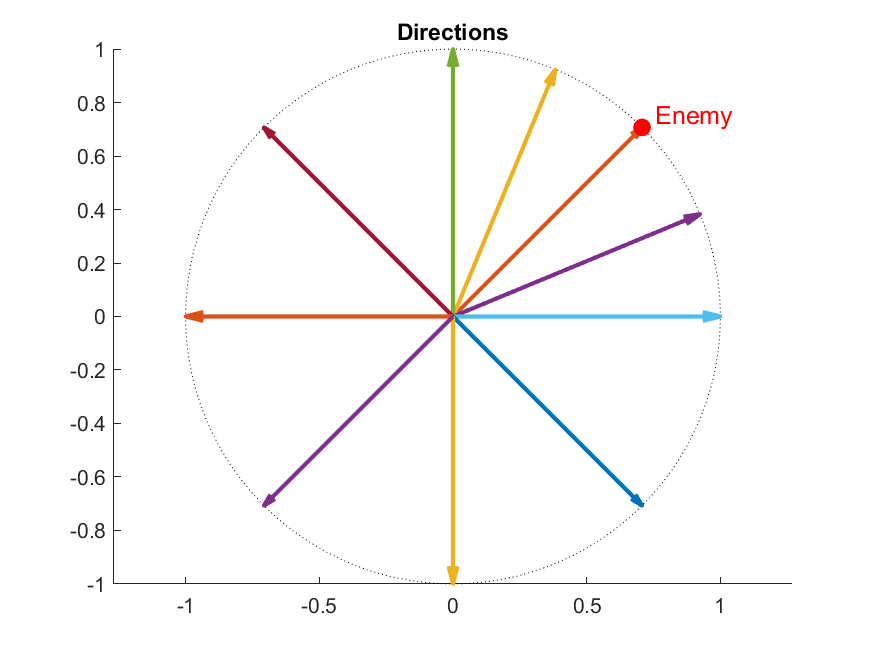
\includegraphics[width=\linewidth]{./assets/directions.png}
\end{minipage}
\vspace{0.5cm}
\\This spell probably needs piercing, scattering into more projectiles, or bouncing to feel impactful. 

\subsection{Fireball}
Common spell.  
\begin{itemize}    
    \item Targeting: Seeks the nearest enemy and explodes.
    \item Range: Ranged. 
    \item Cooldown: Frequent.
    \item Scaling: Increases damage and explosion radius. 
    \item Status Effects: Knockback and DoT to all enemies in the explosion radius.
\end{itemize}

\subsection{Magic Missile}
Common spell.  
\begin{itemize}
    \item Targeting: Seeks the nearest enemy. 
    \item Range: Ranged. 
    \item Cooldown: Frequent.
    \item Scaling: Increases damage and fires additional missiles (each targeting a different enemy). 
    \item Status Effects: Small knockback. 
\end{itemize}

\subsection{Lightning}
Common spell.  
\begin{itemize}
    \item Targeting: Strikes the nearest enemy and chains to others.
    \item Range: Ranged. 
    \item Cooldown: Frequent.
    \item Scaling: Increases damage and the number of bounces.
    \item Status Effects: Chance to stun enemies.
\end{itemize}

\subsection{Celestial Orbs}
Common spell.  
\begin{itemize}
    \item Targeting: Creates orbs that hover around the player.
    \item Range: Mid-range. 
    \item Cooldown: Once (or do they vanish over time?).
    \item Scaling: Increases damage and the number of orbs.
    \item Status Effects: Knockback.
\end{itemize}

\subsection{Discussion}
Each spell likely requires its own systems for shooting, collision detection, and dealing damage.  
How do spells level up? Do we want spells to combine with each other? 

\end{document}